\documentclass{scrartcl}
\usepackage{collect}

\definecollection{answers}

\newcommand\mycollect[1]{%
  \collect{answers}
    {\par\medskip\noindent\جواب~#1}
    {\par}
    {}{}%
}

\newenvironment{answer}
  {\begingroup\edef\x{\endgroup\noexpand\mycollect{\theexercise}}\x}
  {\endcollect}

\newcounter{exercise}
\newenvironment{ex}
  {\refstepcounter{exercise}\par\noindent سوال~\theexercise}
  {\par}

\begin{document}

\begin{ex}
$x^2=\sin t$
\begin{answer}
$x=\sin t\cos t$
\end{answer}
\end{ex}
\begin{ex}
\end{ex}
\begin{answer}
\begin{center}
%	x^2+4z^2=16
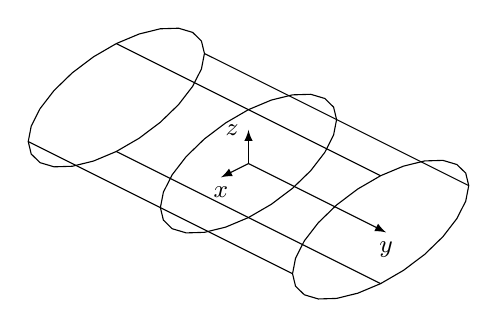
\begin{tikzpicture}[font=\small,declare function={fx(\r,\t)=4*\r*cos(\t);fz(\r,\t)=2*\r*sin(\t);}]
\pgfmathsetmacro{\ta}{0}
\pgfmathsetmacro{\tb}{90}
\pgfmathsetmacro{\tc}{180}
\pgfmathsetmacro{\td}{270}
\pgfmathsetmacro{\ky}{12}
\begin{axis}[view/h=135,axis equal,axis lines=center,xtick={\empty},ytick={\empty},ztick={\empty},xlabel={$x$},ylabel={$y$},zlabel={$z$},xlabel style={anchor=east},ylabel style={anchor=west},zlabel style={anchor=east},
axis x line=none,axis y line=none,axis z line=none]
\addplot3[domain y=0:360] ({fx(2,y)},-\ky,{fz(2,y)});
\addplot3[domain y=0:360] ({fx(2,y)},0,{fz(2,y)});
\addplot3[domain y=0:360] ({fx(2,y)},\ky,{fz(2,y)});
\addplot3[] coordinates {({fx(2,\ta)},-\ky,{fz(2,\ta)})({fx(2,\ta)},\ky,{fz(2,\ta)})};
\addplot3[] coordinates {({fx(2,\tb)},-\ky,{fz(2,\tb)})({fx(2,\tb)},\ky,{fz(2,\tb)})};
\addplot3[] coordinates {({fx(2,\tc)},-\ky,{fz(2,\tc)})({fx(2,\tc)},\ky,{fz(2,\tc)})};
\addplot3[] coordinates {({fx(2,\td)},-\ky,{fz(2,\td)})({fx(2,\td)},\ky,{fz(2,\td)})};
\addplot3[-latex] coordinates {(0,0,0)(2.5,0,0)}node[below]{$x$};
\addplot3[-latex] coordinates {(0,0,0)(0,\ky+0.5,0)}node[below]{$y$};
\addplot3[-latex] coordinates {(0,0,0)(0,0,2.5)}node[left]{$z$};
\end{axis}
\end{tikzpicture}
\end{center}

\end{answer}

\begin{ex}
\end{ex}
\begin{answer}
کیا حال ہے
\end{answer}



\includecollection{answers}

\end{document}
